\documentclass[11pt,aspectratio=16:9]{beamer}

\usetheme{Madrid}
\usecolortheme{default}
\setbeamertemplate{navigation symbols}{}

% Packages
\usepackage{graphicx}
\usepackage{amsmath}
\usepackage{amssymb}
\usepackage{xcolor}
\usepackage{tikz}
\usepackage{array}
\usepackage{booktabs}

% Custom colors
\definecolor{darkblue}{RGB}{0,51,102}
\definecolor{lightblue}{RGB}{135,206,235}
\definecolor{darkgreen}{RGB}{34,139,34}
\definecolor{accentcolor}{RGB}{200,100,50}

% Title and author info
\title{Legal Query System}
\subtitle{A RAG-Based Legal Document Intelligence Platform}
\author{Group Project}
\date{\today}

\begin{document}

% Title Slide
\begin{frame}
    \titlepage
    \vspace{-1cm}
    \begin{center}
        {\small Full-Stack RAG Application for Legal Document Analysis}
    \end{center}
\end{frame}

% Outline
\begin{frame}{Outline}
    \tableofcontents
\end{frame}

% ==================== SECTION 1: PROJECT OVERVIEW ====================
\section{Project Overview}

\begin{frame}{What is the Legal Query System?}
    \begin{columns}
        \column{0.5\textwidth}
        \textbf{Core Purpose:}
        \begin{itemize}
            \item AI-powered legal document search
            \item Retrieves relevant legal sections automatically
            \item Generates contextual answers with citations
            \item Multi-turn conversation support
        \end{itemize}
        
        \column{0.5\textwidth}
        \textbf{Key Features:}
        \begin{itemize}
            \item Semantic search (not keyword matching)
            \item Proper source citations
            \item User authentication
            \item Session management
            \item Real-time responses
        \end{itemize}
    \end{columns}
    
    \vspace{0.5cm}
    \hrule
    \vspace{0.5cm}
    
    {\small \textit{Think of it as "ChatGPT for Indian Legal Documents"}}
\end{frame}

\begin{frame}{Project Goals}
    \begin{enumerate}
        \item \textbf{Accessibility:} Make legal information searchable for everyone
        \item \textbf{Accuracy:} Provide citations to source documents
        \item \textbf{Scalability:} Handle large legal document collections
        \item \textbf{User Experience:} Simple, intuitive interface
        \item \textbf{Security:} Protect user data and conversations
    \end{enumerate}
    
    \vspace{0.8cm}
    
    \begin{center}
        \fcolorbox{darkblue}{lightblue!30}{\parbox{0.8\textwidth}{
            \textbf{Challenge:} Making AI-generated legal answers trustworthy and verifiable
        }}
    \end{center}
\end{frame}

% ==================== SECTION 2: ARCHITECTURE ====================
\section{System Architecture}

\begin{frame}{Three-Layer Architecture}
    \begin{center}
        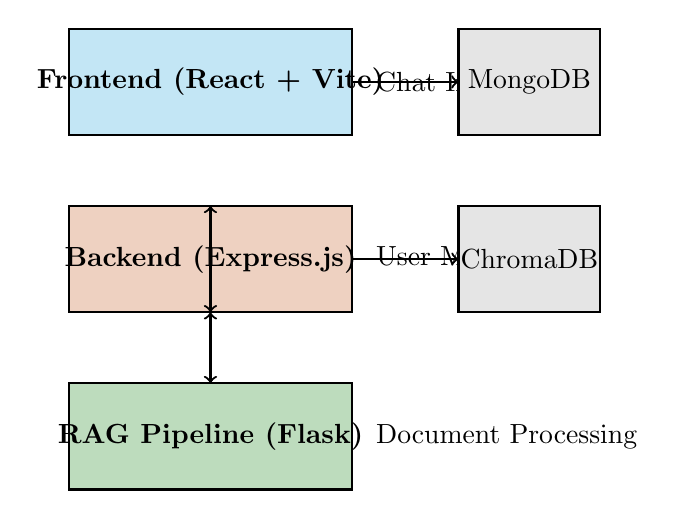
\begin{tikzpicture}[scale=0.9]
            % Frontend Layer
            \draw[fill=lightblue!50, thick] (0,5) rectangle (4,6.5);
            \node at (2,5.75) {\textbf{Frontend (React + Vite)}};
            \node[right] at (4.2,5.75) {Chat Interface};
            
            % Backend Layer
            \draw[fill=accentcolor!30, thick] (0,2.5) rectangle (4,4);
            \node at (2,3.25) {\textbf{Backend (Express.js)}};
            \node[right] at (4.2,3.25) {User Management};
            
            % RAG Pipeline Layer
            \draw[fill=darkgreen!30, thick] (0,0) rectangle (4,1.5);
            \node at (2,0.75) {\textbf{RAG Pipeline (Flask)}}; 
            \node[right] at (4.2,0.75) {Document Processing};
            
            % Databases
            \draw[fill=gray!20, thick] (5.5, 5) rectangle (7.5, 6.5);
            \node at (6.5,5.75) {MongoDB};
            
            \draw[fill=gray!20, thick] (5.5, 2.5) rectangle (7.5, 4);
            \node at (6.5,3.25) {ChromaDB};
            
            % Arrows
            \draw[->, thick] (4, 5.75) -- (5.5, 5.75);
            \draw[->, thick] (4, 3.25) -- (5.5, 3.25);
            \draw[<->, thick] (2, 4) -- (2, 2.5);
            \draw[<->, thick] (2, 2.5) -- (2, 1.5);
        \end{tikzpicture}
    \end{center}
    
    \vspace{0.5cm}
    {\small All components communicate via REST APIs}
\end{frame}

\begin{frame}{Frontend: User Interface}
    \textbf{React + Vite Stack}
    
    \begin{columns}
        \column{0.5\textwidth}
        \textbf{Pages:}
        \begin{itemize}
            \item \texttt{/login} - Authentication
            \item \texttt{/signup} - Registration
            \item \texttt{/dashboard} - Session list
            \item \texttt{/chat/:id} - Chat interface
        \end{itemize}
        
        \column{0.5\textwidth}
        \textbf{Key Components:}
        \begin{itemize}
            \item Protected routes
            \item JWT token management
            \item Real-time message display
            \item Citation cards
        \end{itemize}
    \end{columns}
    
    \vspace{0.8cm}
    
    {\small \fbox{User types query $\to$ Frontend sends to Backend $\to$ Results displayed}}
\end{frame}

\begin{frame}{Backend: API Server}
    \textbf{Express.js + MongoDB}
    
    \begin{columns}
        \column{0.5\textwidth}
        \textbf{Responsibilities:}
        \begin{itemize}
            \item User authentication
            \item Chat session management
            \item Query coordination
            \item Data persistence
        \end{itemize}
        
        \column{0.5\textwidth}
        \textbf{Key Endpoints:}
        \begin{itemize}
            \item \texttt{POST /auth/login}
            \item \texttt{GET /chat/sessions}
            \item \texttt{POST /chat/query}
            \item \texttt{DELETE /chat/:id}
        \end{itemize}
    \end{columns}
    
    \vspace{0.5cm}
    
    \begin{center}
        \textbf{Security Features:}
        \begin{itemize}
            \item JWT authentication (HS256)
            \item Bcrypt password hashing (12 salt rounds)
            \item User isolation (can only access own sessions)
            \item Input validation
        \end{itemize}
    \end{center}
\end{frame}

\begin{frame}{RAG Pipeline: The Intelligence Layer}
    \textbf{Retrieval-Augmented Generation (Flask)}
    
    \begin{center}
        \textbf{Query Processing Flow:}
        \vspace{0.3cm}
        
        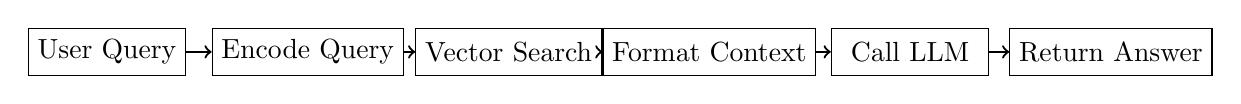
\begin{tikzpicture}[scale=0.85]
            \node [draw, rectangle, minimum width=2cm, minimum height=0.6cm] (query) at (0,0) {User Query};
            \node [draw, rectangle, minimum width=2cm, minimum height=0.6cm] (encode) at (3,0) {Encode Query};
            \node [draw, rectangle, minimum width=2cm, minimum height=0.6cm] (search) at (6,0) {Vector Search};
            \node [draw, rectangle, minimum width=2cm, minimum height=0.6cm] (format) at (9,0) {Format Context};
            \node [draw, rectangle, minimum width=2cm, minimum height=0.6cm] (llm) at (12,0) {Call LLM};
            \node [draw, rectangle, minimum width=2cm, minimum height=0.6cm] (response) at (15,0) {Return Answer};
            
            \draw[->, thick] (query) -- (encode);
            \draw[->, thick] (encode) -- (search);
            \draw[->, thick] (search) -- (format);
            \draw[->, thick] (format) -- (llm);
            \draw[->, thick] (llm) -- (response);
        \end{tikzpicture}
    \end{center}
    
    \vspace{0.8cm}
    
    \textbf{Technologies:}
    \begin{itemize}
        \item \textbf{Embeddings:} Sentence-Transformers (all-MiniLM-L6-v2) - 384-dim vectors
        \item \textbf{Vector DB:} ChromaDB with cosine similarity search
        \item \textbf{LLM:} Google Vertex AI Gemini 2.0 Flash
        \item \textbf{Context Window:} Last 6 messages + top-6 relevant chunks
    \end{itemize}
\end{frame}

% ==================== SECTION 3: DOCUMENT PROCESSING ====================
\section{Document Processing}

\begin{frame}{Document Ingestion Pipeline}
    \textbf{How we prepare legal documents for searching:}
    
    \vspace{0.5cm}
    
    \begin{enumerate}
        \item \textbf{PDF Extraction} - PyPDF2 parses PDFs, preserves page markers
        \item \textbf{Smart Chunking} - Splits by legal sections (Section 3A, Rule 22, etc.)
        \item \textbf{Metadata Tagging} - Adds act name, section number, chapter info
        \item \textbf{Vector Embedding} - Converts text chunks to 384-dim vectors
        \item \textbf{Indexing} - Stores in ChromaDB for fast similarity search
    \end{enumerate}
    
    \vspace{0.8cm}
    
    \begin{center}
        \small
        PDF Files → Extracted Text → Legal Chunks → Embeddings → ChromaDB Index
    \end{center}
    
    \vspace{0.5cm}
    {\small \textit{Performance: ~2000 legal sections indexed in 5-10 seconds}}
\end{frame}

\begin{frame}{Smart Legal Chunking Strategy}
    \textbf{Why not just split by word count?}
    
    \begin{columns}
        \column{0.5\textwidth}
        \textbf{Naive Approach:}
        \begin{itemize}
            \item [--] Splits sections arbitrarily
            \item [--] Loses legal context
            \item [--] Bad for citations
            \item [--] Confusing for users
        \end{itemize}
        
        \column{0.5\textwidth}
        \textbf{Our Approach:}
        \begin{itemize}
            \item [+] Respects legal structure
            \item [+] Keeps context intact
            \item [+] Clear citations
            \item [+] Semantic coherence
        \end{itemize}
    \end{columns}
    
    \vspace{0.8cm}
    
    \textbf{Implementation:}
    \begin{itemize}
        \item Detect section headers: "Section 33A", "Rule 5", "Chapter II", etc.
        \item Split on these boundaries
        \item For very long sections ($>$2000 words): split into 400-word parts with 50-word overlap
        \item Preserve metadata: act name, section number, chapter, page numbers
    \end{itemize}
\end{frame}

\begin{frame}{Metadata for Perfect Citations}
    \textbf{Each chunk stores rich metadata:}
    
    \vspace{0.5cm}
    
    \begin{center}
        \small
        \begin{tabular}{ll}
            chunk\_id & IT\_2000\_SEC\_33A \\
            text & Section 33A. Web portal of certifying authority... \\
            act\_name & Information Technology Act \\
            act\_year & 2000 \\
            section\_number & 33A \\
            section\_title & Power of controller \\
            chapter & VI \\
            page\_number & 42 \\
            similarity\_score & 0.92 \\
        \end{tabular}
    \end{center}
    
    \vspace{0.5cm}
    {\small This metadata is used to generate proper citations in responses}
\end{frame}

% ==================== SECTION 4: RETRIEVAL & GENERATION ====================
\section{Query Processing}

\begin{frame}{How a Query Gets Answered}
    \textbf{Complete journey of a user's question:}
    
    \vspace{0.3cm}
    
    \begin{small}
    \begin{enumerate}
        \item User types: \texttt{"What are the penalties for cybercrime?"}
        \item Frontend sends query to Express backend
        \item Express validates JWT token, finds user's session
        \item Forwards to Flask RAG API with chat history
        \item RAG pipeline converts query to vector (using same embedding model)
        \item Searches ChromaDB: "Find top-6 most similar chunk vectors"
        \item Retrieves: IT Act Sec 43, 43A, 65, etc. (sorted by relevance)
        \item Formats retrieved chunks with citations
        \item Sends to Gemini LLM: \textit{"Here are 6 relevant law sections. Based on these, answer the user's question with proper citations."}
        \item LLM generates answer with citations
        \item Express saves to MongoDB (user message + assistant response)
        \item Frontend displays answer with expandable source cards
    \end{enumerate}
    \end{small}
    
    \vspace{0.5cm}
    {\textbf{Total latency: ~2-3 seconds}}
\end{frame}

\begin{frame}{Retrieval: Semantic Search}
    \textbf{Why semantic search beats keyword matching:}
    
    \vspace{0.5cm}
    
    \begin{columns}
        \column{0.5\textwidth}
        \textbf{Keyword Search:}
        \begin{itemize}
            \item Q: "crime on internet"
            \item Only finds "crime" + "internet"
            \item Misses related sections
        \end{itemize}
        
        \column{0.5\textwidth}
        \textbf{Semantic Search:}
        \begin{itemize}
            \item Q: "crime on internet"
            \item Finds cybercrime, hacking, phishing, etc.
            \item Understands meaning
        \end{itemize}
    \end{columns}
    
    \vspace{0.8cm}
    
    \textbf{Our Implementation:}
    \begin{itemize}
        \item Embedding Model: \textbf{Sentence-Transformers all-MiniLM-L6-v2}
        \item Output: 384-dimensional vector (compact \& fast)
        \item Search: Cosine similarity in ChromaDB
        \item Top Results: Retrieve top-6 chunks
        \item Filtering: Exclude results with $<30\%$ similarity
    \end{itemize}
\end{frame}

\begin{frame}{Generation: Creating Accurate Responses}
    \textbf{How we ensure trustworthy AI responses:}
    
    \vspace{0.5cm}
    
    \textbf{LLM Configuration:}
    \begin{itemize}
        \item \textbf{Model:} Google Vertex AI Gemini 2.0 Flash
        \item \textbf{Temperature:} 0.2 (deterministic, not creative)
        \item \textbf{Max Tokens:} 2048 (balanced detail \& conciseness)
        \item \textbf{Context Window:} 32K tokens (enough for legal docs)
    \end{itemize}
    
    \vspace{0.5cm}
    
    \textbf{Prompt Engineering:}
    \begin{itemize}
        \item System message: "You are a legal assistant. Always cite sources."
        \item Always include source references in response
        \item Add disclaimer: "This is AI-generated. Consult actual lawyer for legal advice."
        \item Refuse to answer beyond retrieved context
    \end{itemize}
    
    \vspace{0.5cm}
    
    {\small \textit{Key insight: We don't let the LLM hallucinate. It can only use info from retrieved documents.}}
\end{frame}

% ==================== SECTION 5: USER EXPERIENCE ====================
\section{User Experience}

\begin{frame}{Authentication Flow}
    \textbf{Secure user access:}
    
    \begin{center}
        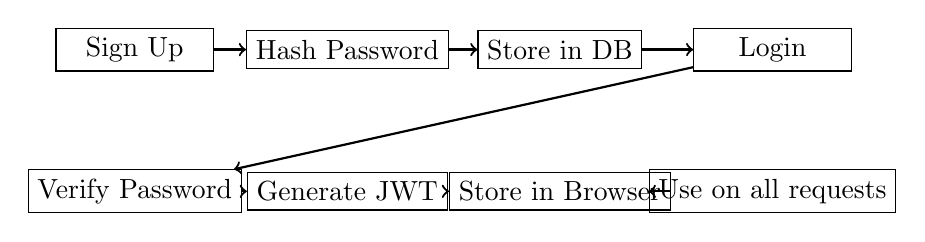
\begin{tikzpicture}[scale=0.9]
            \node [draw, rectangle, minimum width=2cm] (signup) at (0,2) {Sign Up};
            \node [draw, rectangle, minimum width=2cm] (hash) at (3,2) {Hash Password};
            \node [draw, rectangle, minimum width=2cm] (store) at (6,2) {Store in DB};
            \node [draw, rectangle, minimum width=2cm] (login) at (9,2) {Login};
            
            \node [draw, rectangle, minimum width=2cm] (verify) at (0,0) {Verify Password};
            \node [draw, rectangle, minimum width=2cm] (jwt) at (3,0) {Generate JWT};
            \node [draw, rectangle, minimum width=2cm] (storage) at (6,0) {Store in Browser};
            \node [draw, rectangle, minimum width=2cm] (use) at (9,0) {Use on all requests};
            
            \draw[->, thick] (signup) -- (hash);
            \draw[->, thick] (hash) -- (store);
            \draw[->, thick] (store) -- (login);
            \draw[->, thick] (login) -- (verify);
            \draw[->, thick] (verify) -- (jwt);
            \draw[->, thick] (jwt) -- (storage);
            \draw[->, thick] (storage) -- (use);
        \end{tikzpicture}
    \end{center}
    
    \vspace{0.5cm}
    
    \textbf{Security Features:}
    \begin{itemize}
        \item Bcrypt 12 salt rounds (passwords never stored plaintext)
        \item JWT tokens (stateless authentication)
        \item 24-hour expiration (automatic re-login)
        \item CORS validation
    \end{itemize}
\end{frame}

\begin{frame}{Dashboard: Session Management}
    \textbf{Users can manage their legal queries:}
    
    \begin{columns}
        \column{0.7\textwidth}
        \textbf{Dashboard Features:}
        \begin{itemize}
            \item List all user's chat sessions
            \item Filter: All, Active, Solved
            \item View: Title, message count, last message
            \item Actions: Open, Edit, Delete, Mark as Solved
            \item Create new query button
        \end{itemize}
        
        \column{0.3\textwidth}
        \small
        \begin{tabular}{|l|}
            \hline
            \textbf{Session 1} \\
            Cybercrime Penalties \\
            5 messages \\
            Active \\
            \hline
            \textbf{Session 2} \\
            Contract Law \\
            12 messages \\
            Solved \\
            \hline
        \end{tabular}
    \end{columns}
    
    \vspace{0.8cm}
    
    \textbf{Data Persistence:} All sessions stored in MongoDB with user ID, so users can resume conversations anytime.
\end{frame}

\begin{frame}{Chat Interface: Multi-Turn Conversations}
    \textbf{Intelligent conversation support:}
    
    \vspace{0.5cm}
    
    \begin{center}
        \small
        \begin{tabular}{|l|p{7cm}|}
            \hline
            \textbf{User:} & "What is Section 33A?" \\
            \hline
            \textbf{Assistant:} & "Section 33A covers web portal requirements... [Citation: IT Act 2000, Section 33A]" \\
            \hline
            \textbf{User:} & "What are the penalties?" \\
            \hline
            \textbf{Assistant:} & "The penalties for violating Section 33A include... [Citation: IT Act 2000, Section 43]" \\
            \hline
        \end{tabular}
    \end{center}
    
    \vspace{0.8cm}
    
    \textbf{How it works:}
    \begin{itemize}
        \item Maintains last 6 messages in context (previous Q\&A)
        \item LLM can reference earlier messages
        \item Coherent follow-up responses
        \item Example: "penalties?" understood as penalty for previous topic
    \end{itemize}
\end{frame}

\begin{frame}{Citation Display}
    \textbf{Expandable source cards show exactly where info came from:}
    
    \vspace{0.5cm}
    
    \small
    \fcolorbox{darkblue}{lightblue!20}{\parbox{0.9\textwidth}{
        \textbf{Answer:} The Information Technology Act, 2000 defines digital signatures for authentication...
    }}
    
    \vspace{0.3cm}
    
    \textbf{Sources (Ranked by Relevance):}
    \begin{enumerate}
        \item \textbf{[92\% match]} IT Act 2000, Section 3 - Scope of application
            \begin{itemize}
                \item {\small "This Act applies to any offense or contravention..."}
            \end{itemize}
        \item \textbf{[87\% match]} IT Act 2000, Section 5 - Interpretation
            \begin{itemize}
                \item {\small "Digital signature means authentication of digital..."}
            \end{itemize}
        \item \textbf{[82\% match]} IT Act 2000, Section 43 - Penalties
    \end{enumerate}
    
    \vspace{0.5cm}
    {\small User can click to expand full text of each source.}
\end{frame}

% ==================== SECTION 6: TECHNICAL DETAILS ====================
\section{Technical Implementation}

\begin{frame}{Technology Stack Summary}
    \begin{center}
        \begin{tabular}{|l|l|l|}
            \hline
            \textbf{Layer} & \textbf{Technology} & \textbf{Key Libraries} \\
            \hline
            Frontend & React 18 + Vite 5 & React Router, Axios, Lucide \\
            \hline
            Backend API & Express 4 + Node.js & Mongoose 8, JWT 9, Bcryptjs \\
            \hline
            RAG Pipeline & Flask 3 + Python 3 & LangChain 0.3, ChromaDB 0.5 \\
            \hline
            Embeddings & Sentence-Transformers & all-MiniLM-L6-v2 (384-dim) \\
            \hline
            Vector DB & ChromaDB 0.5 & Local SQLite backend \\
            \hline
            LLM & Google Vertex AI & Gemini 2.0 Flash \\
            \hline
            Databases & NoSQL & MongoDB (users/chats) \\
            \hline
        \end{tabular}
    \end{center}
    
    \vspace{0.5cm}
    {\small All components communicate via REST APIs with JSON payloads}
\end{frame}

\begin{frame}{Performance Metrics}
    \textbf{How fast is the system?}
    
    \vspace{0.5cm}
    
    \begin{columns}
        \column{0.5\textwidth}
        \textbf{Ingestion Phase:}
        \begin{itemize}
            \item PDF parsing: $<$1s
            \item Chunking: $<$1s
            \item Embedding: $\sim$3-5s
            \item Total: 5-10s for 2000 sections
        \end{itemize}
        
        \column{0.5\textwidth}
        \textbf{Query Phase:}
        \begin{itemize}
            \item Vector search: $<$100ms
            \item Context formatting: $<$50ms
            \item LLM inference: $\sim$1-2s
            \item Database save: $<$100ms
        \end{itemize}
    \end{columns}
    
    \vspace{0.8cm}
    
    \begin{center}
        \fcolorbox{darkgreen}{lightblue!20}{\parbox{0.8\textwidth}{
            \textbf{End-to-End Query Response: ~2-3 seconds}
        }}
    \end{center}
    
    \vspace{0.5cm}
    {\small LLM inference dominates latency; vector search is negligible}
\end{frame}

\begin{frame}{Security Architecture}
    \textbf{How we protect user data:}
    
    \vspace{0.5cm}
    
    \begin{itemize}
        \item \textbf{Password Security:} Bcrypt 12 salt rounds (slow by design)
        \item \textbf{Authentication:} JWT tokens with HS256 signature
        \item \textbf{API Protection:} JWT middleware on all protected endpoints
        \item \textbf{Data Isolation:} MongoDB queries filtered by userId
        \item \textbf{CORS:} Only trusted domains can access API
        \item \textbf{Input Validation:} Sanitize all user inputs
        \item \textbf{No PII Logging:} Don't log sensitive data
        \item \textbf{Timeout:} JWT expires after 24 hours
    \end{itemize}
    
    \vspace{0.8cm}
    
    {\small \textbf{Result: Each user can only access their own sessions}}
\end{frame}

% ==================== SECTION 7: CHALLENGES & SOLUTIONS ====================
\section{Challenges \& Solutions}

\begin{frame}{Challenge 1: LLM Hallucinations}
    \textbf{Problem:} AI might make up legal information
    
    \vspace{0.5cm}
    
    \textbf{Our Solution:}
    \begin{itemize}
        \item \textbf{Constrain Context:} Only let LLM use retrieved chunks
        \item \textbf{System Prompt:} "Refuse to speculate beyond provided sources"
        \item \textbf{Disclaimer:} Always add: "This is AI-generated. Consult a lawyer."
        \item \textbf{Cite Everything:} Every claim must have a source
        \item \textbf{Low Temperature:} Set to 0.2 (deterministic, not creative)
        \item \textbf{Relevance Filter:} Exclude sources $<30\%$ similar
    \end{itemize}
    
    \vspace{0.5cm}
    
    \textbf{Result:} Responses are grounded in actual law documents
\end{frame}

\begin{frame}{Challenge 2: Semantic Relevance}
    \textbf{Problem:} "What's cybercrime?" vs "What is hacking?" are related
    
    \vspace{0.5cm}
    
    \textbf{Our Solution:}
    \begin{itemize}
        \item \textbf{Embeddings:} Use pre-trained Sentence-Transformers
        \item \textbf{Multilingual:} Model trained on legal documents + general corpus
        \item \textbf{384 Dimensions:} Balance between expressiveness \& speed
        \item \textbf{Cosine Similarity:} Measures semantic closeness
        \item \textbf{Top-6 Results:} Provides diverse perspectives
    \end{itemize}
    
    \vspace{0.5cm}
    
    \textbf{Result:} Semantic matching instead of keyword matching
\end{frame}

\begin{frame}{Challenge 3: Legal Document Structure}
    \textbf{Problem:} Sections are semantically important; can't just split by word count
    
    \vspace{0.5cm}
    
    \textbf{Our Solution:}
    \begin{itemize}
        \item \textbf{Domain-Aware Chunking:} Detect "Section X", "Rule Y" patterns
        \item \textbf{Preserve Hierarchy:} Keep act/chapter/section structure
        \item \textbf{Metadata Tags:} Store act year, section number, page refs
        \item \textbf{Overlapping Chunks:} Large sections overlap for context
        \item \textbf{Adaptive Sizing:} 400-500 words typical, up to 2000 words for large sections
    \end{itemize}
    
    \vspace{0.5cm}
    
    \textbf{Result:} Better retrieval quality + accurate citations
\end{frame}

\begin{frame}{Challenge 4: Scalability}
    \textbf{Problem:} As documents/users grow, system slows down
    
    \vspace{0.5cm}
    
    \textbf{Current Setup:}
    \begin{itemize}
        \item Single Express instance
        \item Single MongoDB instance
        \item Single Flask RAG server
    \end{itemize}
    
    \vspace{0.5cm}
    
    \textbf{Future Scaling:}
    \begin{itemize}
        \item \textbf{Load Balancer:} Nginx/HAProxy to distribute requests
        \item \textbf{Horizontal Database:} MongoDB replica sets \& sharding
        \item \textbf{Multiple RAG Instances:} Redis queue for job distribution
        \item \textbf{Distributed Vectors:} Pinecone/Weaviate for massive embeddings
        \item \textbf{Caching:} Redis for frequent queries
        \item \textbf{CDN:} Cloudflare for static assets
    \end{itemize}
    
    \vspace{0.3cm}
    {\small Can scale from 10 concurrent users to 1000+ users}
\end{frame}

% ==================== SECTION 8: PROJECT PROGRESS ====================
\section{Project Status}

\begin{frame}{What We've Completed}
    \begin{itemize}
        \item [+] \textbf{RAG Pipeline:} Full document ingestion + query engine
        \item [+] \textbf{Backend API:} Express.js with all endpoints
        \item [+] \textbf{Frontend:} React UI with authentication
        \item [+] \textbf{Database:} MongoDB + ChromaDB setup
        \item [+] \textbf{Vector Search:} Semantic search working
        \item [+] \textbf{LLM Integration:} Gemini 2.0 Flash connected
        \item [+] \textbf{Authentication:} JWT + Bcrypt implemented
        \item [+] \textbf{Multi-Turn Conversations:} Chat history working
        \item [+] \textbf{Citation Tracking:} Source references displayed
        \item [+] \textbf{Error Handling:} Graceful degradation
    \end{itemize}
\end{frame}

\begin{frame}{Project Statistics}
    \begin{center}
        \begin{tabular}{|l|r|}
            \hline
            \textbf{Metric} & \textbf{Value} \\
            \hline
            Total Lines of Code & $\sim$3000+ \\
            Backend Endpoints & 10+ \\
            Frontend Routes & 4 \\
            Database Collections & 3 \\
            Vector Embeddings Indexed & 2000+ \\
            \hline
            Python Files & 3 \\
            JavaScript Files & 8+ \\
            JSON Config Files & 5+ \\
            \hline
            Development Hours & $\sim$60+ \\
            Integration Points & 15+ \\
            API Calls per Query & 4-5 \\
            \hline
        \end{tabular}
    \end{center}
\end{frame}

\begin{frame}{Future Enhancements}
    \textbf{Short-Term (Next 1-2 weeks):}
    \begin{itemize}
        \item Advanced filtering (by date, jurisdiction, document type)
        \item Query analytics dashboard
        \item PDF export of chat sessions
        \item User feedback system
    \end{itemize}
    
    \vspace{0.4cm}
    
    \textbf{Medium-Term (1-3 months):}
    \begin{itemize}
        \item Document upload feature for users
        \item Multi-language legal systems support
        \item LLM fine-tuning on legal corpus
        \item Comparison tools (compare sections)
        \item Smart summarization
    \end{itemize}
    
    \vspace{0.4cm}
    
    \textbf{Long-Term (3-6 months):}
    \begin{itemize}
        \item Multi-modal support (OCR for scanned documents)
        \item Real-time collaboration
        \item Third-party integrations
        \item Mobile applications
        \item API for external developers
    \end{itemize}
\end{frame}

% ==================== CLOSING ====================
\section*{Conclusion}

\begin{frame}{Key Takeaways}
    \begin{enumerate}
        \item \textbf{RAG is Powerful:} Combining retrieval + LLM creation makes trustworthy AI
        \item \textbf{Domain Knowledge Matters:} Understanding legal docs $\rightarrow$ better chunking
        \item \textbf{Citations Build Trust:} Users can verify AI responses against sources
        \item \textbf{Architecture Scales:} Three-layer design supports growth
        \item \textbf{Security First:} JWT + Bcrypt protect user data
        \item \textbf{UX is Important:} Simple interface $>$ fancy features
    \end{enumerate}
\end{frame}

\begin{frame}[plain]
    \begin{center}
        \Huge \textbf{Thank You!}
        
        \vspace{1cm}
        
        \Large Legal Query System \\
        \large AI-Powered Legal Document Intelligence
        
        \vspace{2cm}
        
        {\footnotesize Questions?}
    \end{center}
\end{frame}

\end{document}
